\section{Pendahuluan}
\indent Internet Protocol Address v6 (IPv6) adalah standar protokol yang digunakan untuk mengidentifikasi
dan mengarahkan alamat jaringan dalam jaringan komputer. Dibandingkan dengan pendahulunya,
IPv4, IPv6 memiliki format alamat yang lebih panjang dengan 128 bit, yang memungkinkan jumlah
alamat yang jauh lebih besar, sehingga dapat mengatasi kekurangan alamat IPv4 yang semakin berkurang. IPv6 juga mendukung fitur-fitur tambahan, termasuk pemantauan aliran lalu lintas, keamanan
yang ditingkatkan, dan kualitas layanan yang lebih baik, menjadikannya solusi jangka panjang untuk
pertumbuhan Internet yang pesat dan kebutuhan alamat yang terus berkembang.


%===========================================================%

\section{Tujuan Praktikum}
\begin{enumerate}
	\item Mengetahui bagaimana konfigurasi static routing menggunakan Ipv6
	\item Mengimplementasikan konfigurasi Ipv6 pada perangkat mikrotik
\end{enumerate}

%===========================================================%

\section{Alat dan Bahan}
\begin{itemize}[label=$\bullet$, itemsep=-1pt, leftmargin=*]
	\item 2 buah Cloud Core Router
	\item 3 Kabel UTP (LAN)
	\item 2 buah Laptop
	\item Software Winbox
\end{itemize}
%===========================================================%

\section{Langkah-langkah Percobaan}
\textbf{gambar pada langkah-langkah di bagian ini akan diisi gambar contoh dari template dulu,
		karena nanti akan kami ganti dengan screenshot langkah-langkah kami saat praktikum}

%Langkah untuk konfigurasi Router 1
\begin{center} 
	\textbf{Konfigurasi PC 1}
\end{center}

\begin{enumerate}
	% poin 1
	\item 
	
	\begin{figure}[H]
		\centering
		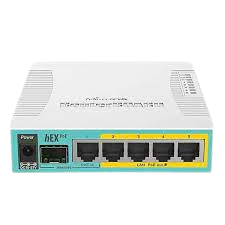
\includegraphics[width=0.7\linewidth]{P1/img/contoh.png}
		\caption{Step 1}
		\label{fig:gambar1}
	\end{figure}

	% poin 2
	\item 
	
	\begin{figure}[H]
		\centering
		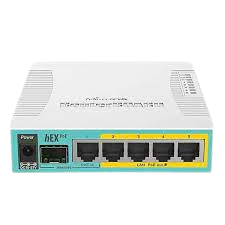
\includegraphics[width=0.7\linewidth]{P1/img/contoh.png}
		\caption{Step 2}
		\label{fig:gambar1}
	\end{figure}

	% poin 3
	\item 
	
	\begin{figure}[H]
		\centering
		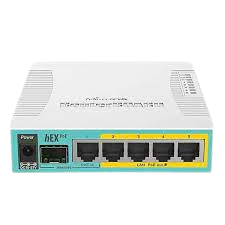
\includegraphics[width=0.7\linewidth]{P1/img/contoh.png}
		\caption{Step 3}
		\label{fig:gambar1}
	\end{figure}

	% poin 4
	\item 
	
	\begin{figure}[H]
		\centering
		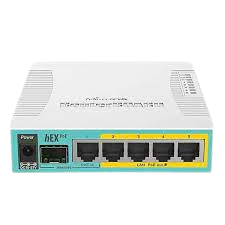
\includegraphics[width=0.7\linewidth]{P1/img/contoh.png}
		\caption{Step 4}
		\label{fig:gambar1}
	\end{figure}

	% poin 5
	\item 
	
	\begin{figure}[H]
		\centering
		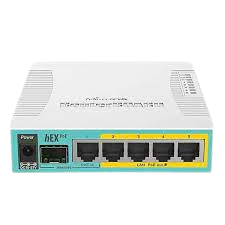
\includegraphics[width=0.7\linewidth]{P1/img/contoh.png}
		\caption{Step 5}
		\label{fig:gambar1}
	\end{figure}

	% poin 6
	\item  	
	
	\begin{figure}[H]
		\centering
		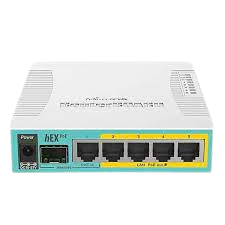
\includegraphics[width=0.7\linewidth]{P1/img/contoh.png}
		\caption{Step 6}
		\label{fig:gambar1}
	\end{figure}

	% poin 7
	\item 
	
	\begin{figure}[H]
		\centering
		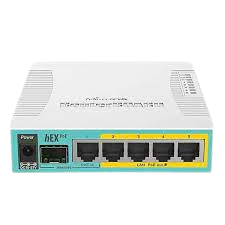
\includegraphics[width=0.7\linewidth]{P1/img/contoh.png}
		\caption{Step 7}
		\label{fig:gambar1}
	\end{figure}

	% poin 8
	\item 
	
	\begin{figure}[H]
		\centering
		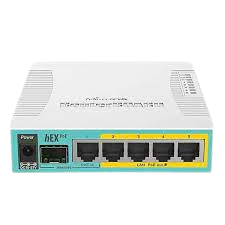
\includegraphics[width=0.7\linewidth]{P1/img/contoh.png}
		\caption{Step 8}
		\label{fig:gambar1}
	\end{figure}

\end{enumerate}

%Langkah untuk konfigurasi Router 2
\begin{center} 
	\textbf{Konfigurasi PC 2}
\end{center}

\begin{enumerate}
	% poin 1
	\item 
	
	\begin{figure}[H]
		\centering
		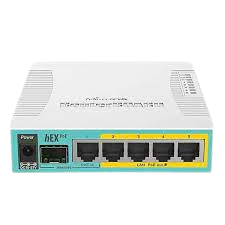
\includegraphics[width=0.7\linewidth]{P1/img/contoh.png}
		\caption{Step 1}
		\label{fig:gambar1}
	\end{figure}

	% poin 2
	\item 	
	
	\begin{figure}[H]
		\centering
		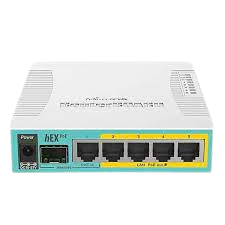
\includegraphics[width=0.7\linewidth]{P1/img/contoh.png}
		\caption{Step 2}
		\label{fig:gambar1}
	\end{figure}

	% poin 3
	\item 
	
	\begin{figure}[H]
		\centering
		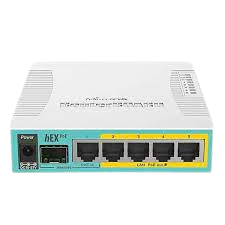
\includegraphics[width=0.7\linewidth]{P1/img/contoh.png}
		\caption{Step 3}
		\label{fig:gambar1}
	\end{figure}

	% poin 4
	\item 
	
	\begin{figure}[H]
		\centering
		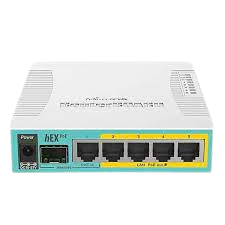
\includegraphics[width=0.7\linewidth]{P1/img/contoh.png}
		\caption{Step 4}
		\label{fig:gambar1}
	\end{figure}

	% poin 5
	\item 
	
	\begin{figure}[H]
		\centering
		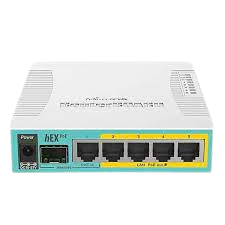
\includegraphics[width=0.7\linewidth]{P1/img/contoh.png}
		\caption{Step 5}
		\label{fig:gambar1}
	\end{figure}

	% poin 6
	\item 
	
	\begin{figure}[H]
		\centering
		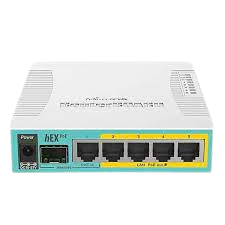
\includegraphics[width=0.7\linewidth]{P1/img/contoh.png}
		\caption{Step 6}
		\label{fig:gambar1}
	\end{figure}

	% poin 7
	\item 
	
	\begin{figure}[H]
		\centering
		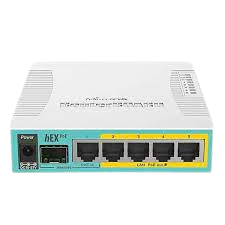
\includegraphics[width=0.7\linewidth]{P1/img/contoh.png}
		\caption{Step 7}
		\label{fig:gambar1}
	\end{figure}

	% poin 8
	\item 
	
	\begin{figure}[H]
		\centering
		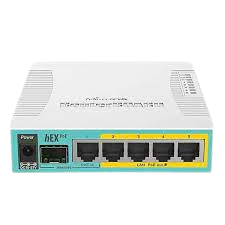
\includegraphics[width=0.7\linewidth]{P1/img/contoh.png}
		\caption{Step 8}
		\label{fig:gambar1}
	\end{figure}

\end{enumerate}

%Langkah untuk Pengujian konfigurasi
\begin{center} 
	\textbf{Pengujian Konfigurasi}
\end{center}

\begin{enumerate}
	% poin 1
	\item 
	
	\begin{figure}[H]
		\centering
		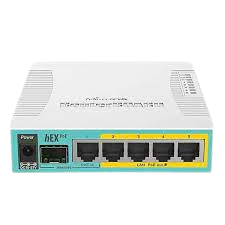
\includegraphics[width=0.7\linewidth]{P1/img/contoh.png}
		\caption{Step 1}
		\label{fig:gambar1}
	\end{figure}

	% poin 2
	\item 	
	
	\begin{figure}[H]
		\centering
		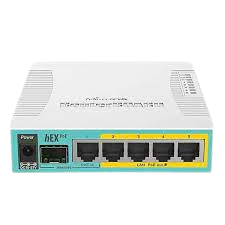
\includegraphics[width=0.7\linewidth]{P1/img/contoh.png}
		\caption{Step 2}
		\label{fig:gambar1}
	\end{figure}

\end{enumerate}

\section{Hasil Percobaan}
akan diisi setelah praktikum
%===========================================================%

\section{Kesimpulan}
akan diisi setelah praktikum
%===========================================================%

\section{Lampiran}

\subsection{Tugas Pendahuluan}
\begin{enumerate}
	\item Apa solusi lain ketika IPv4 habis, selain menggunakan IPv6?
	
	\begin{itemize}
		\item Network Address Translation (NAT): \\ NAT memungkinkan banyak perangkat dalam jaringan lokal untuk berbagi satu alamat IPv4 publik. Ini memperlambat laju kehabisan alamat IPv4 dengan memungkinkan penggunaan kembali alamat yang sama oleh banyak perangkat di jaringan yang berbeda.
		\item Carrier-Grade NAT (CGNAT): \\ CGNAT adalah versi NAT yang diterapkan oleh penyedia layanan internet (ISP) pada skala yang lebih besar. Ini memungkinkan ISP untuk mengelola dan membagi alamat IPv4 publik di antara banyak pelanggan, menghemat alamat IPv4.
		\item Reclaiming dan reallocating Alamat IPv4: \\ Memulihkan dan mendistribusikan kembali alamat IPv4 yang tidak digunakan atau tidak dialokasikan secara optimal. Ini melibatkan audit dan pemulihan blok alamat yang mungkin dialokasikan tetapi tidak digunakan secara aktif.
		\item Protokol dan Teknologi Penghematan IP: \\ Mengembangkan dan menggunakan protokol baru yang lebih hemat dalam penggunaan alamat IP, seperti Tunneling Protocols yang memungkinkan penggunaan alamat IPv4 dalam lingkungan IPv6, atau teknologi seperti Multiprotocol Label Switching (MPLS).
	\end{itemize}

	\item Sebutkan tiga keunggulan IPv6 dibandingkan IPv4!
	
	\begin{itemize}
		\item Keunggulan IPv6 :
		\begin{itemize}
			\item[\ding{58}] Cepat \\ karena IPv6 tak lagi bergantung kepada Network Address Translation (NAT) sehingga mempercepat proses pengiriman data. Terlebih lagi jika pada perangkat mobile akan dapat lebih cepat karena koneksinya tidak harus melewati NAT.
			\item[\ding{58}] Efektif \\ karena ukuran routing table lebih kecil dibanding IPv4, maka proses routing dapat lebih sistematis dan tentunya efektif.
			\item[\ding{58}] Aman \\ IPv6 sudah dapat menghindari serangan ke ARP (address resolution protocol) yang dapat mengalihkan lalu lintas jaringan kemudian mengalihkannya.
			\item[\ding{58}] Hemat Bandwidth \\ penggunaan bandwidth dapat lebih hemat karena sudah mendukung multicast.
			\item[\ding{58}] Konfigurasi yang Mudah \\ IPv6 sudah mendukung konfigurasi secara otomatis, sehingga dapat lebih memudahkan dan menghemat waktu.
		\end{itemize}
	\end{itemize}

	\item Mengapa panjang awal alamat IPv6 biasanya adalah 128 bit?
	\\ \indent IPv6 menggunakan desain ruang alamat yang berbeda dari IPv4. IPv6 menggunakan subnetting untuk meningkatkan efisiensi pemanfaatan ruang alamat kecil, sehingga ruang alamat IPv6 dianggap cukup besar untuk masa mendatang. 
	Dengan 128 bit, IPv6 dapat menyediakan sekitar $2^{128}$ alamat unik yang cukup untuk mendukung pertumbuhan internet dalam jangka panjang dan menghindari masalah kehabisan alamat yang dialami dengan IPv4.

\end{enumerate}

\subsection{Dokumentasi saat Praktikum}
akan diisi setelah praktikum
\begin{figure}[H]
	\centering
	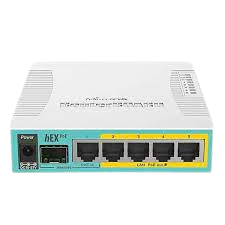
\includegraphics[width=0.75\linewidth]{P1/img/contoh.png}
	\caption{Dokumentasi saat praktikum}
	\label{fig:gambar32}
\end{figure}